%%%%%%%%%%%%%%%%%%%%%%%%%%%%%%%%%%%%%%%%%%%%%
%IB pdf source code written by bear blinschauer
%using Stylish article template 

% http://www.LaTeXTemplates.com
% License:
% CC BY-NC-SA 3.0 (http://creativecommons.org/licenses/by-nc-sa/3.0/)

%this project itself wont have a lisence because it will never
%see the light of day after grading and is not profitable
%%%%%%%%%%%%%%%%%%%%%%%%%%%%%%%%%%%%%%%%%%%%%


%----------------------------------------------------------------------------------------
%	PACKAGES AND OTHER DOCUMENT CONFIGURATIONS
%----------------------------------------------------------------------------------------

\documentclass[fleqn,10pt]{SelfArx} % Document font size and equations flushed left

\usepackage[english]{babel} % Specify a different language here - english by default
\usepackage {graphicx, animate}
\usepackage{csquotes}
\usepackage[style=ieee,backend=biber]{biblatex}
\addbibresource{MathIA.bib}

%----------------------------------------------------------------------------------------
%	COLUMNS
%----------------------------------------------------------------------------------------

\setlength{\columnsep}{0.55cm} % Distance between the two columns of text
\setlength{\fboxrule}{0.75pt} % Width of the border around the abstract

%----------------------------------------------------------------------------------------
%	COLORS
%----------------------------------------------------------------------------------------

\definecolor{color1}{RGB}{0,0,90} % Color of the article title and sections
\definecolor{color2}{RGB}{0,20,20} % Color of the boxes behind the abstract and headings

%----------------------------------------------------------------------------------------
%	HYPERLINKS
%----------------------------------------------------------------------------------------

\usepackage{hyperref} % Required for hyperlinks

\hypersetup{
	hidelinks,
	colorlinks,
	breaklinks=true,
	urlcolor=color2,
	citecolor=color1,
	linkcolor=color1,
	bookmarksopen=false,
	pdftitle={Title},
	pdfauthor={Author},
}

%----------------------------------------------------------------------------------------
%	ARTICLE INFORMATION
%----------------------------------------------------------------------------------------

\JournalInfo{Analysis and Approaches, Collis, 2024} % Journal information
\Archive{} % Additional notes (e.g. copyright, DOI, review/research article)

\PaperTitle{Math IA 2024\\Rotation Using Matrix Math} % Article title

\Authors{Bear BlinSchauer} % Authors

\Keywords{} % Keywords - if you don't want any simply remove all the text between the curly brackets
\newcommand{\keywordname}{Keywords} % Defines the keywords heading name

\setlength\parindent{24pt}

%----------------------------------------------------------------------------------------
%	ABSTRACT
%----------------------------------------------------------------------------------------

\Abstract{abstract goes here.}

%----------------------------------------------------------------------------------------

\begin{document}

\maketitle % Output the title and abstract box

\tableofcontents % Output the contents section

\thispagestyle{empty} % Removes page numbering from the first page

%----------------------------------------------------------------------------------------
%	ARTICLE CONTENTS
%----------------------------------------------------------------------------------------
\section*{Introduction}

\addcontentsline{toc}{section}{Introduction} % Adds this section to the table of contents

\hspace{\parindent}
IB often pushes people to create projects that connect to their personal life or interests. As an individual I am fascinated by 3d graphics and research the topic on my own time. I think that mathematical applications in computer graphics is a fascinating part of both computer science and math. The idea that math is able to describe entire virtual environments is incredible. There is a multitude of different parts of math used in 3d graphics but in this essay I will research vectors and rotational transformation.

Often while trying to learn graphics I get roadblocked by rotation vectors and the triginometry inside the function appears intimidating. In this math Internal Assesment I decided to learn how rotation matrices work using the unit circle and implement the algorithm into a simple program that rotates a triangle 3-dimensionally. This essay will connect to triginometry because I will utilize basic triginometry to reason vector composition and I will use the unit circle in order to visualize rotation.

This essay connects to personal acedemic ventures of mine. As a side project I wish to write a renderer on my computer. I believe that it is important as a learner to understand how to make transformations in three dimensional space because it allows the individual to make an end product more intuitively and to work in 3d space without any help or helper libraries.

In this project I hope to write about the proccess of triginometry applied to rotation in three dimensional space. During this project I will be writing a program applying the math with the end goal of getting a triangle to rotate in 3d space on my screen.\\
\begin{math}
\overset{\rightarrow}{v}=\begin{bmatrix} x \\ y \end{bmatrix}
\end{math}

\section{Problem}
% \addcontentsline{toc}{section}{Problem} % Adds this section to the table of contents


% \href{http://www.google.de}{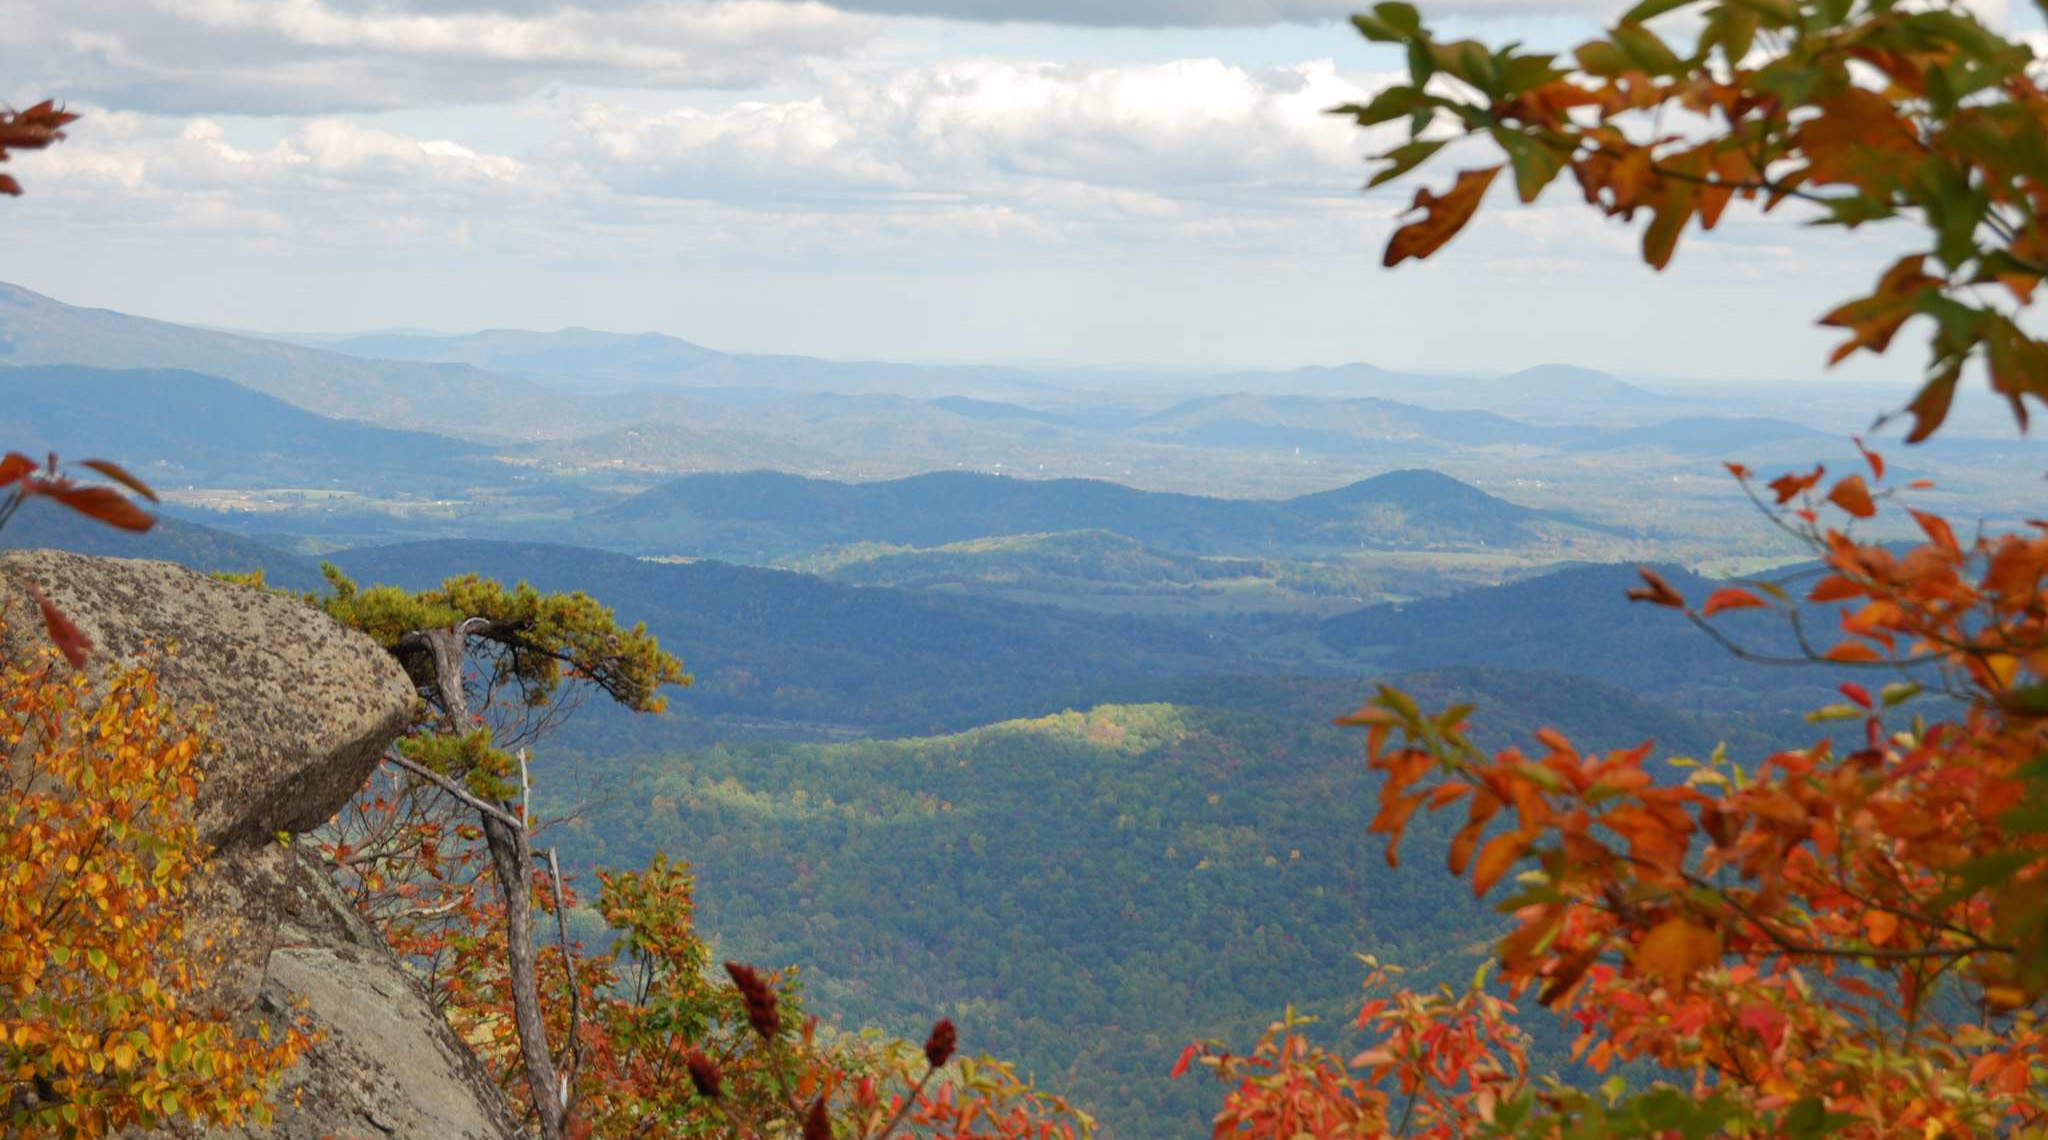
\includegraphics[width=\linewidth]{view}}% [1]
%adobe sucks just give up and link to raw github content
% \animategraphics[scale=0.4,loop,autoplay]{30}{Figures/monkeyRotation/foo-}{0}{99}
% \noindent\animategraphics[scale=0.9,controls,step]{0}{animate}{}{}



%----------------------------------------------------------------------------------------
%	REFERENCE LIST
%----------------------------------------------------------------------------------------
\autocite{dr_peyam_rotation_2019}
\phantomsection
\nocite{*}
\begin{flushleft}
  \printbibliography
\end{flushleft}
% \printbibliography
% \bibliographystyle{unsrt}
% \bibliography{MathIA.bib}

%----------------------------------------------------------------------------------------

\end{document}
